% !TEX program = xelatex
\chapter{Kamerasysteme}
\label{ch:hardware}
\section{Kamerasensoren}
  \begin{figure}
    \centering
    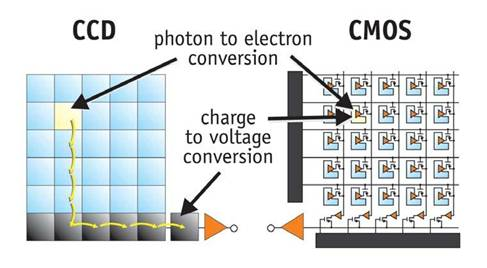
\includegraphics[width=0.75\textwidth]{pictures/04_CCD_CMOS.jpg}
    \caption[Aufbau CCD vs CMOS]{Aufbau CCD vs CMOS (Merolini, 2022 \cite{Merolini.IMG})}
    \label{fig:ccdcmos}
  \end{figure}

  Um eine Schätzung der Pose eines Fahrzeugs in seiner Umgebung vornehmen zu können, muss ein Modell der Umgebung erstellt werden. Kamerasensoren sind externe Sensoren die Eigenschaften und Informationen der Umwelt erfassen.
  \newline  

  Kamerasensoren sind mittlerweile preisgünstig, während die Qualität und Auflösung der Bilder hoch ist. Dadurch sind sie einer breiten Masse von Forschern und Studenten zugänglich, auch ein Grund ist warum visuelle Bildverarbeitungssysteme in der Robotik so verbreitet sind. 
  \newline
  
  Um die Kamerapose durch Visuelle Odometrie zu schätzen muss in jedem Fall ein Weg gefunden werden Informationen über die Distanz zwischen der Kamera und Objekten aus der Umgebung zu gewinnen. Die Tiefe kann mit einer einzelnen Kamera rein algorithmisch geschätzt werden. Mit zwei Kameras lässt sich durch Stereoskopie ein Sonderfall der Epipolargeometrie ausnutzen und Punkte können effizient trianguliert werden. Spezielle Tiefenbildkameras mit Infrarot (IR) Projektion oder Time-of-Flight (ToF) Messungen lösen das Problem vollständig in Hardware. Im folgenden soll auf die wichtigsten Sensoren kurz eingegangen werden.


  \subsection{RGB Kamera mit CCD- oder CMOS-Sensoren}

  \subsubsection{CCD Sensoren}
  Die CCD Technologie wurde Mitte der 70er Jahre erfunden. CCD war damals der Durchbruch der Halbleitersensoren. Die Abkürzung CCD steht dabei für "Charge-Coupled Device".
  \newline
  
  Aufgrund der Funktionsweise des Ladungsträgertransportes werden sie oft mit Eimerketten verglichen. Eine Elektronenschicht liegt auf einer Fotozellen Silizium-Trägerschicht. Auf die Fotozelle einfallendes Licht löst negativ geladene Elektronen aus den Silizium Atomen. Je intensiver das Licht, desto mehr Elektronen lösen sich. Jede Fotozelle ist mit einem Gate verbunden. An das Gate wird eine Spannung angelegt, wodurch die Ladung angezogen werden. Durch gezieltes heben und senken des Potentials werden die Ladungsträger durch die Speicherbereiche geschoben. Die Ladung wandert solange durch das Array, bis der Rand des Sensors erreicht ist. Dort wird das Ladungspaket von einem externen Verstärker in eine Spannung konvertiert.


  CCD ist zeichnet sich durch eine hohe Bildqualität aus. Die Frequenz, mit der der Ladungsträgertransport durchgeführt werden kann, ist jedoch begrenzt und niedriger als bei CMOS. Bei zu hohen Frequenzen würde im CCD zu viel Ladung verloren gehen.
  Das Verschieben der Ladungsträger in CCD Sensoren kann au{\ss}erdem zum sog. Blooming Effekt führen, der bei CMOS Sensoren nicht auftritt.

  \subsubsection{CMOS Sensoren}

  Complementary Metal-Oxide Semiconductor, kurz CMOS, Sensoren sind ebenfalls bereits seid en 1970er Jahren auf dem Markt. Es dauerte jedoch noch einige Jahrzehnte bis die CMOS Technologie die heutige Bildqualität erreichte. Da CMOS-Sensoren neben der hohe Bildraten mittlerweile auch eine gute Bildqualität vorweisen, verdrängen sie CCD-Sensoren aus den meisten Anwendungen. 
  \newline

  Während CCD die Ladungspakete extern in Spannung konvertiert, wird die Ladung bei CMOS bereits im Pixel umgewandelt. CMOS Sensoren die selbst Ladung konvertieren werden deshalb auch als Aktiver Pixel Sensor (APS) bezeichnet.

\begin{figure}[h!]
  \centering
  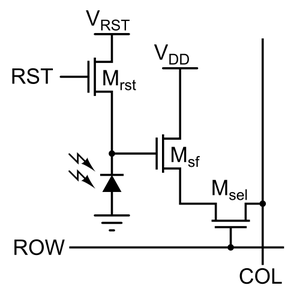
\includegraphics[width=0.4\textwidth]{04_CMOS_3T_circuit.png}
  \caption[3 Transistor CMOS Schaltung]{Schaltung eines einfachen 3 Transistor aktiven Pixels (Wikimedia Creative Commons \cite{Wikimedia})}
  \label{fig:cmos}
\end{figure}

  Ein Einfaches CMOS-Sensor Pixel besteht aus drei MOSFETs und einer Photodiode wie in \ref{fig:cmos} gezeigt. $M_{sf}$ agiert als Verstärker, $M_{rst}$ als Reset der Photodiode und mit $M_{sel}$ kann die Reihe ausgewählt werden.
  \newline

  Wird der Reset geöffnet, erzeugt die Photodiode je nach einfallender Lichtintensität Spannung am Verstärker. Die Spannung wird über den SEL Transistor ausgelesen. 
  \newline

  Wird ein Bild von einem Objekt aufgenommen, das sich in Bewegung befindet, kann es zum sog. Rolling-Shutter Effekt kommen. Durch eine minimale zeitliche Verzögerung bei der Belichtung der Reihen tritt eine Verzerrung im Bild auf. Der Effekt wird Behoben indem zwei weitere Transistoren und ein Kondensator in die Pixelzelle hinzugefügt werden. Dadurch können alle Photodioden zur selben Zeit zurückgesetzt werden und die Belichtungszeit wird synchronisiert.
    

\subsection{Tiefenbildkameras auf Basis von Projektionen}

Das Bekannteste Beispiel dieses Kameratyps ist wohl die ursprünglich für die XBox Spielekonsole eingeführt Kinect 1 Kamera. Ein IR-Transmitter sendet ein bekanntes Muster aus, das von einem Receiver wieder empfangen wird. Objekte auf die das Muster trifft reflektieren das Muster. Je nach Beschaffenheit und Entfernung des Objekts ist das Empfangende Muster Verzerrt und anders skaliert. 
\newline

Das Erfassen von Entfernung durch Musterprojektionen ist sehr empfindlich gegenüber Fremdlicht und hat nur eine begrenzte Genauigkeit. Es gibt daher auch den Ansatz Projektion mit Stereoskopie zu kombinieren wie beispielsweise bei Intels D400 Serie. Neben einer höheren Reichweite ist die Motivation für die IR Projektion hier vor allem ein Nachteil der Stereokamera auszugleichen. Finden sich keine markanten Strukturen im Bild, beispielsweise bei einer wei{\ss}en Wand, kann Stereoskopie versagen. Für solche Fälle führt eine Fusion aus Stereoskopie und Projektion, zumindest Indoor (Reichweite 4m), zu wesentlich Robusteren Ergebnissen. \cite{realsense}

\subsection{Tiefenbildkameras auf Basis von Stereoskopie}

Bei Stereokameras sind zwei Kameras exakt parallel zueinander Ausgerichtet und um eine Baseline b verschoben. Aus der Epipolargeometrie folgt, dass in diesem Fall die Epipole im unendlichen liegen. D.h. die Epipolarlinien verlaufen auf gleicher Höhe durch die Bildebenen der beiden Kameras. Das bedeutet, der Suchraum eines Punktes aus dem linken Kamerabild ist im Rechten Kamerabild enorm beschränkt. Wurde die Abbildung des Punktes in beiden Bildebenen gefunden kann direkt trianguliert werden, da die Baseline bereits bekannt ist. Auf diese weise wird ein Tiefenprofil erstellt. Stereokameras nutzen Kamerasensoren und haben eine entsprechend gro{\ss}e Reichweite. 

\subsection{Time-of-Flight Tiefenbild}

Time-of-Flight Kameras verwenden Photonic Mixing Device (PMD) Sensoren um über ein Laufzeitverfahren die Distanz zwischen Objekten und Kamera zu messen. Zur Laufzeitmessung wird ein gepulster Infrarot Laserstrahl ausgesendet und von einem Receiver empfangen. Dabei wird durch die Phasenverschiebung des Pulses gemessen wie viel Zeit zwischen Senden und Empfangen vergangen ist. Da die Laufzeit von Licht bekannt ist, kann so auf die zurückgelegt Distanz des Laserpulses geschlossen werden.
\begin{equation}
  \centering
  t_D = 2 \cdot \frac{D}{c}
\end{equation}

Mit $t_D$ Zeit, $D$ Distanz und $c$ Lichtgeschwindigkeit $\approx 300\, 000\: \frac{km}{s}$.
\newline

\section{Kamerakonfigurationen}
Da die Visuelle Odometrie auf Kameradaten basiert stellt sich auch die Frage, wie viele Kameras benötigt werden. Grundsätzlich können eine, zwei oder mehrere Kameras beliebig am Fahrzeug montiert werden. Aber nicht jeder Aufbau ist effizient oder sinnvoll.
\newline

Durchgesetzt hat sich monokulare Visuelle Odometrie mit einer Kamera und stereo VO mit zwei Kameras. In dem Versuch die Robustheit von Visueller Odometrie zu erhöhen, vor allem in schlecht belichteten Umgebungen wurden auch Mehrkamerasysteme mit mehr als zwei Kameras untersucht. Liu et al. untersuchten 2019 ein Multi-Stereokamera Setup \cite{mulVO_2019} und erzielten bessere Ergebnisse für Nachtfahrten mit einem Offline-Dataset. Mhiri et al. veröffentlichten bereits 2014 eine Methode in der sie Visuelle Odometrie mit klassischer SfM und Machine Learning kombinierten um die Odometrie aus einem Mehrkamerasystem mit zu schätzen, bei dem die Kameras nicht synchronisiert wurden \cite{Mhiri_2014}.

Mehrkamerasysteme sind eine Seltenheit um sehr spezielle Problemstellungen zu lösen. Weitaus häufiger wird Visuelle Odometrie durch Sensorfusion mit anderen Sensoren kombiniert um dei Robustheit zu erhöhen. Es sit au{\ss}erdem zu beobachten, dass der Trend in die entgegengesetzte Richtung geht. Viele, in den letzten Jahren veröffentlichte Paper, untersuchen monokulare Visuelle Odometrie. Monokulare Visuelle Odometrie ist bereits so lange bekannt wie Stereo Visuelle Odometrie, mittlerweile ist die Technik jedoch weit genug fortgeschritten um monokulare Systeme mit Neuronale Netze (lernende Visuelle Odometrie Verfahren) zu implementieren, welche die Nachteile von monokularen Systemen beheben sollen.   

\subsection{Monokulare Kamerasysteme}
Bei monokularen Kamerasystemen wird die Odometrie anhand aufeinanderfolgender Bilder einer einzelnen Kamera geschätzt. Der Vorteil dabei ist, das weniger Hardware benötigt wird. Das grö{\ss}te Problem ist die Tiefenschätzung. Ohne eine bekannte Basislinie, wie bei Stereokameras, muss die Skalierung zwischen den Bildern ebenfalls geschätzt werden. Dadurch erhöht sich die Drift des Systems. Monokulare und Stereo Visuelle Odometrie haben sich über die Zeit als zwei unterschiedliche Forschungsgebiete entwickelt. Dennoch kann monokulare Visuelle Odometrie auch für stereo Visuelle Odometrie interessant werden, wenn der Abstand zu Szene wesentlich grö{\ss}er als die Basislinie ist. In dem Fall wird aus der stereo eine mono Visuelle Odometrie. Für autonome Fahrzeuge trifft dieser Fall i.d.R. nicht ein.   


\subsection{Stereo Kamerasysteme}
Stereokameras setzen sich aus zwei Kameras zusammen, die exakt parallel ausgerichtet sind und eine feste Basislinie haben. Der Grund dafür sind die besonderen Eigenschaften der Epipolargeometrie solch eines Aufbaus. Dadurch können Pixel schnell Trianguliert werden und so eine Tiefenkarte aus der Geometrie geschätzt werden. Stereokameras sind günstig, liefern qualitativ hochwertige Bilder und sind seid Markteinführung der Kinect Kamera auch bei Robotik Enthusiasten verbreitet. 
\begin{figure}[!ht]
  \centering
  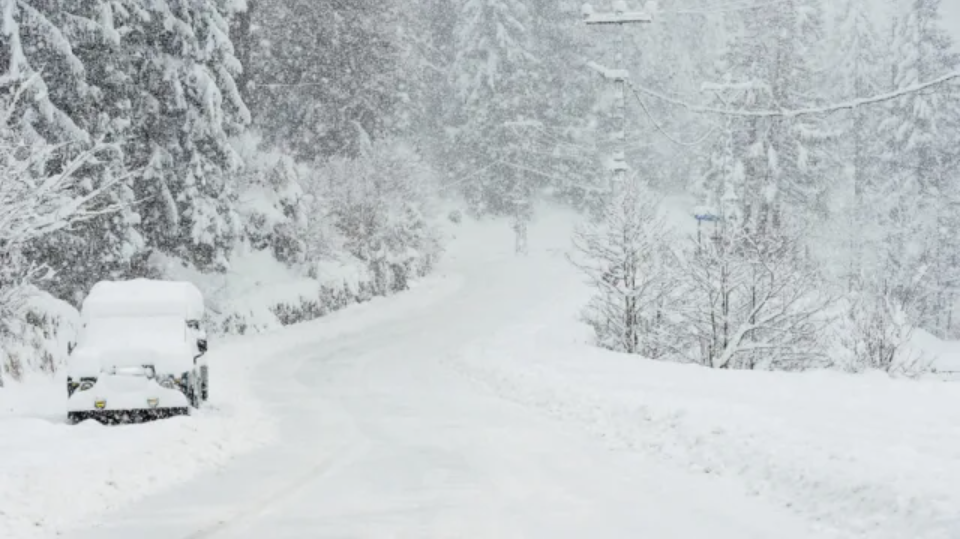
\includegraphics[width=0.75\textwidth]{04_snow.png}
  \caption[Verschneite Stra{\ss}e]{Szenen mit wenig Textur sind auch bei ausreichender Beleuchtung eine Herausforderung für Stereokamera Triangulation (Shutterstock ID 1248440977, 2022)}
\end{figure}
Auch wenn die Triangulation ein schnelles und Zuverlässiges Verfahren ist, muss die abgebildete Szene bestimmte Voraussetzungen Erfüllen. Ohne ausreichende Beleuchtung oder Textur arme Umgebungen führen dazu, dass Pixel nicht abgeglichen werden könne. Ohne ein erfolgreiches Matching kann die Triangulation nicht stattfinden.  


\subsection{RGB mit Tiefenbildkamera}
Für ein Kamerasystem mit RGB-D Kamera wird der gleiche Odometrie Algorithmus implementiert wie für Stereokameras. Software seitig gibt es lediglich den Unterschied, dass das Stereo-Matching und die Triangulation entfällt. Falls diese Schritte nicht ohnehin bereits im Kamerasystem abgearbeitet wurden.

Theoretisch kann eine RGB-D Kamera dort Datenpunkte liefern, wo eine reguläre Stereokamera versagt. Schlechte Lichtverhältnisse und wenig Struktur im Bild haben keine negativen Auswirkungen. Genauso wie sich wiederholende Muster und Asphalt kein Problem darstellen. Dafür wird RGB-D aufgrund des Infrarotlasers durch Sonneneinstrahlung und Reflexionen von Spiegelnden Oberflächen gestört. Dazu kommt, dass die meisten RGB-D Kameras nur über eine geringe Reichweite von wenigen Metern verfügen. In der Praxis werden sie daher überwiegend in geschlossenen Räumen verwendet. In den letzten Jahren kamen jedoch bereits ein paar Kameras auf den Markt, die speziell für den SLAM Einsatz entwickelt wurden und grö{\ss}ere Reichweiten versprechen \cite{rgbd}.

\subsection{Rektifizierung}
\begin{figure}[!ht]
  \centering
  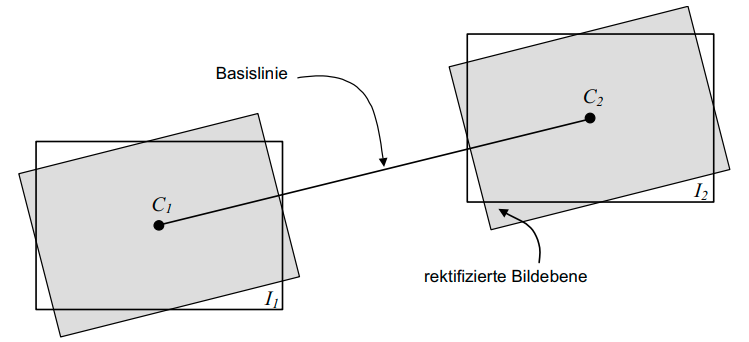
\includegraphics[width=.75\textwidth]{04_rekti2.png}
  \caption[Rektifikation der Stereobildebenen]{Bildebenen einer Stereokamera werden Rektifiziert. Dadurch verlaufen die Epipolarlinien parallel zu den Bildzeilen. (Scheer, 2005 \cite{stereoSchreer})}
\end{figure}
   
Das simulierte Stereokamerasystem das in CARLA am Fahrzeug angebracht wird ist ideal. Alle Kameraparameter sind aus der Konfiguration bekannt. Zwischen der linken und rechten Kamera gibt es keine ungewollte Verschiebung. In realen Systeme sind Stereokameraufbauten i.d.R. nur näherungsweise parallel.

Deshalb werden die Bilder durch eine softwareseitige Drehung in ein tatsächlich achsenparalleles System transformiert. Dieses virtuelle Drehen wird als Rektifizierung bezeichnet und die Kamerabilder als rektifiziert. Die Transformation ist linear und bei erfolgreich transformierten Stereobilder liegen die Epipole im unendlichen. 

Für eine Rektifikation müssen die internen Kameraparameter bekannt sein. Diese sog. intrinsischen Parameter liefert entweder der Kamerahersteller oder werden durch Kamerakalibrierung ermittelt. Wichtig ist zudem, dass sich die Kamerazentren $(C_1 , C_2)$ durch die Rektifizierung nicht verschieben. 